\documentclass[10pt,a4paper]{beamer}

\usepackage[utf8]{inputenc}
\usepackage[russian]{babel}
\usepackage[OT1]{fontenc}
\usepackage{amsmath}
\usepackage{amsfonts}
\usepackage{amssymb}
\usepackage{makeidx}
\usepackage{graphicx}
\usepackage{xcolor}
\usepackage{multirow}

\titlegraphic{
   
\includegraphics[width=4cm]{images/sfera.jpg}
}

\author{Николай Анохин \and Михаил Фирулик}
\title{Введение в Data Science \\ Занятие 1. Классификация и регрессия}

\beamertemplatenavigationsymbolsempty

\begin{document}

\maketitle

\logo{
    
\includegraphics[width=4cm,keepaspectratio]{images/sfera.jpg}\hspace{0.45em}
}

\begin{frame}

\tableofcontents

\end{frame}

% ============================================== %

\section{Постановка задач классификации и регрессии}

% ============================================== %

\begin{frame}{Классификация: интуиция}

\begin{block}{Задача}
Разработать алгоритм, позволяющий определить класс произвольного объекта из некоторго множества
\begin{itemize}
\item Дана {\it обучающая выборка}, в которой для каждого объекта известен класс
\end{itemize}
\end{block} 

\begin{center}
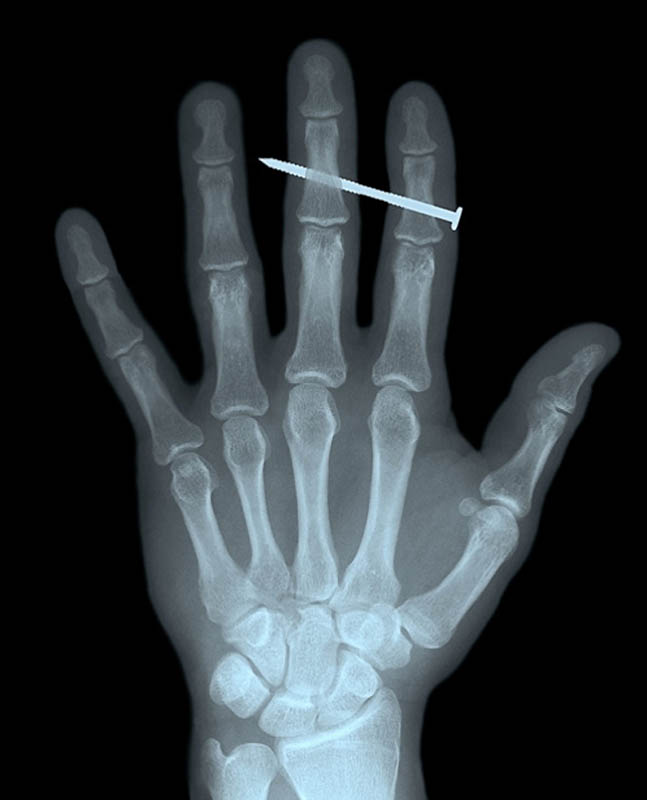
\includegraphics[scale=0.15]{images/xray.jpg}
\end{center}

\end{frame}

% ============================================== %

\begin{frame}{Регрессия: интуиция}

\begin{block}{Задача}
Разработать алгоритм, позволяющий предсказать числовую характеристику произвольного объекта из некоторого множества
\begin{itemize}
\item Дана {\it обучающая выборка}, в которой для каждого объекта известно значение данной числовой характеристики
\end{itemize}
\end{block}

\begin{center}
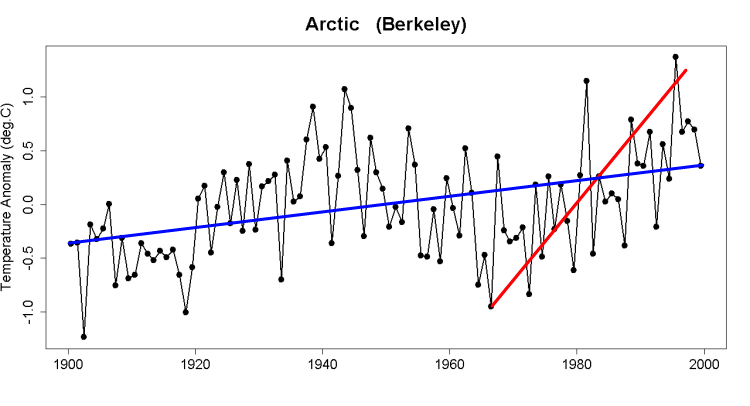
\includegraphics[scale=0.3]{images/kioto.png}
\end{center}

\end{frame}

% ============================================== %

\begin{frame}{Формализуем}

$X$ -- множество объектов \\
$T$ -- множество значений целевой переменной (target variable) 
\vspace{1em}

Дана обучающая выборка из объектов
\[
\boldsymbol X = (x_1, \ldots, x_N)^\top, \; x_i \in X
\]
и соответствующие им классы 
\[
\boldsymbol T = (t_1, \ldots, t_N)^\top, \; t_i \in T
\]

Требуется найти функцию 
\[
y^*(x): X \rightarrow T,
\] 
позволяющую для произвольного $x \in X$ наиболее точно предсказать соответствующее $t \in T$

\end{frame}

% ============================================== %

\begin{frame}{Целевая переменная}

\begin{itemize}
\item $T = \{C_1, \ldots, C_K\}$ -- задача классификации в $K$ непересекающихся классов
\item $T = [a, b] \subset R $ -- задача регрессии
\end{itemize}


\end{frame}

\begin{frame}{Как решать?}

\begin{enumerate}

\item[M] Выдвигаем гипотезу насчет {\bf модели} - семейства параметрических функций вида
\[
Y = \{ y(x, \theta) : X \times \Theta \rightarrow T \},
\]
которая могла бы решить нашу задачу (model selection)

\item[L] Выбираем наилучшие параметры модели $\theta^*$, используя {\bf алгоритм обучения}
\[
A(\boldsymbol X, \boldsymbol T) : (X, T)^N \rightarrow Y
\]
(learning/inference)

\item[D] Используя полученную модель $y^*(x) = y(x, \theta^*)$, классифицируем неизвестные объекты (decision making)

\end{enumerate}

\end{frame}

% ============================================== %

\section{Теория принятия решений}

% ============================================== %

\begin{frame}{Теория принятия решений}

\begin{enumerate}

\item[M] {\color{gray} Выдвигаем гипотезу насчет {\bf модели} - семейства параметрических функций вида
\[
Y = \{ y(x, \theta) : X \times \Theta \rightarrow T \},
\]
которая могла бы решить нашу задачу (model selection)}

\item[L] {\color{gray} Выбираем наилучшие параметры модели $\theta^*$, используя {\bf алгоритм обучения}
\[
A(\boldsymbol X, \boldsymbol T) : (X, T)^N \rightarrow Y
\]
(learning/inference)}

\item[D] {Используя полученную модель $y^*(x) = y(x, \theta^*)$, классифицируем неизвестные объекты (decision making)}

\end{enumerate}

\end{frame}

% ============================================== %

\begin{frame}{Что моделировать?}

{\bf Генеративные модели.} Смоделировать $p(x | C_k)$ и $p(C_k)$, применить теорему Байеса
\[
p(C_k | x) = \frac{p(x | C_k) p(C_k)}{p(x)}
\]
и использовать $p(C_k | x)$ для принятия решения \\ (NB, Bayes Networks, MRF)
\vspace{1em}

{\bf Дискриминативные модели.} Смоделировать $p(C_k | x)$ и использовать ее для принятия решения \\ (Logistic Regression, Decision Trees)
\vspace{1em}

{\bf Функции решения.} Смоделировать напрямую $f(x): X \rightarrow T$ \\ (Linear Models, Neural Networks)

\end{frame}

% ============================================== %

\begin{frame}{Минимизируем риск}

{\bf Пусть}

$\mathcal{R}_k$ -- область, такая что все $x \in \mathcal{R}_k$ относим к $C_k$

{\bf Дано}

$R_{kj}$ -- риск, связанный с отнесением объекта класса $C_k$ к классу $C_j$

{\bf Найти}

$\forall k: \mathcal{R}_k$, такие, что математическое ожидание риска $E[R]$ минимально.

\[
E[R] = \sum_k \sum_j \int_{\mathcal{R}_j} R_{kj} p(C_k | x) p(x) dx
\]

\end{frame}

% ============================================== %

\begin{frame}{Медицинская диагностика}

Матрица риска $[R_{kj}]$

\begin{center}
\begin{tabular}{r | c c}
 & sick & normal \\
\hline
sick & 0 & 10 \\
normal & 1 & 0 
\end{tabular}
\end{center}

Условные вероятности $p(C_k | x)$
\[ 
p(\mathtt{normal} | \mathtt{moving}) = 0.9, \; p(\mathtt{normal} | {\mathtt{not\;moving}}) = 0.3
\]
Вероятности $p(x)$
\[
p(\mathtt{moving}) = 0.7
\]
Требуется определить $\mathcal{R}_{\mathtt{sick}}$, $\mathcal{R}_{\mathtt{normal}}$

\end{frame}

% ============================================== %

\begin{frame}{Регрессия}

Те же виды моделей: {\bf генеративные}, {\bf дискриминативные}, {\bf функция решения}
\vspace{1em}

Задана функция риска
\[
R(t, y(x))
\]
Математическое ожидание $E[R]$
\[
E[R] = \int \!\! \int R(t, y(x)) p(x, t) dx dt 
\]
Для квадратичной функции риска $R(t, y(x)) = [t - y(x)]^2$
\[
y(x) = E_t[t | x]
\]

\end{frame}

% ============================================== %

\begin{frame}{Когда удобнее вероятностные модели}

\begin{itemize}

\item Функция риска может меняться
\item Отказ от классификации (reject option)
\item Дисбаланс в выборке
\item Ансамбли моделей

\end{itemize}

\end{frame}

% ============================================== %

\section{Обучение модели}

% ============================================== %

\begin{frame}{Обучение модели}

% ============================================== %

\begin{enumerate}

\item[M] {\color{gray} Выдвигаем гипотезу насчет {\bf модели} - семейства параметрических функций вида
\[
Y = \{ y(x, \theta) : X \times \Theta \rightarrow T \},
\]
которая могла бы решить нашу задачу (model selection)}

\item[L] {Выбираем наилучшие параметры модели $\theta^*$, используя {\bf алгоритм обучения}
\[
A(\boldsymbol X, \boldsymbol T) : (X, T)^N \rightarrow Y
\]
(learning/inference)}

\item[D] {\color{gray} Используя полученную модель $y^*(x) = y(x, \theta^*)$, классифицируем неизвестные объекты (decision making)}

\end{enumerate}

\end{frame}

% ============================================== %

\begin{frame}{Выбор параметров модели}

{\bf Функция потерь} $\mathcal{L}(x, t, \theta)$ - ошибка, которую для данного $x$ дает модель $y(x, \theta)$ по сравнению с реальным значением $t$
\vspace{1em}

{\bf Эмпирический риск} -- средняя ошибка на обучающей выборке
\[
Q(\boldsymbol X, \boldsymbol T, \theta) = \frac{1}{N} \sum_{k=1}^N \mathcal{L}(x_k, t_k, \theta)
\]
\vspace{1em}

{\bf Задача} -- найти значение $\theta^*$, минимизирующее эмпирический риск
\[
\theta^* = \theta^*(\boldsymbol X, \boldsymbol T) = \text{argmin}_\theta Q(\boldsymbol X, \boldsymbol T, \theta)
\]

\end{frame}

% ============================================== %

\begin{frame}{Некоторые функции потерь}

\begin{itemize}
\item Индикатор ошибки
\[
\mathcal{L}(x, t, \theta) = 0 \text{\;if\;} y(x, \theta)  = t \text{\;else\;} 1
\]
\item Функция Минковского 
\[
\mathcal{L}(x, t, \theta) = |t - y(x, \theta)|^q
\]
Частные случаи: квадратичная $q = 2$, абсолютная ошибка $q = 1$
\item Hinge
\[
\mathcal{L}(x, t, \theta) = \max(0, 1 - t * y(x, \theta))
\]
\item Информационная
\[
\mathcal{L}(x, t, \theta) = - \log_2 p(t | x, \theta)
\]
\begin{center}

\end{center}
\end{itemize}

\end{frame}

% ============================================== %

\begin{frame}{Проблема 1. Переобучение}

\begin{block}{Задача}
Аппроксимировать обучающую выборку полиномом $M$ степени
\end{block}

\begin{center}
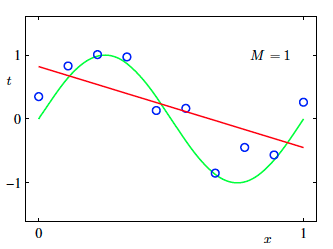
\includegraphics[scale=0.3]{images/m1.png}
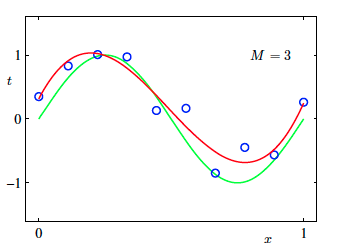
\includegraphics[scale=0.3]{images/m2.png}
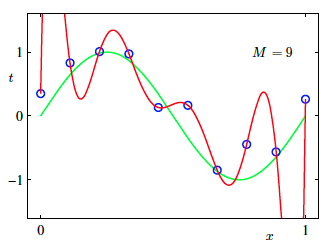
\includegraphics[scale=0.3]{images/m3.png}

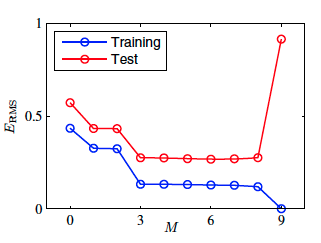
\includegraphics[scale=0.3]{images/of.png}
\end{center}

\end{frame}

% ============================================== %

\begin{frame}{Проблема 2. Проклятие размерности}

\begin{block}{Задача}
Классифицировать объекты.
\end{block}

\begin{center}
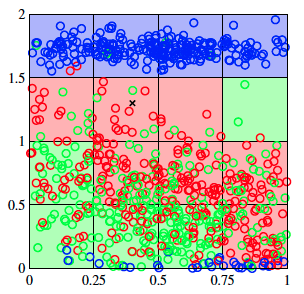
\includegraphics[scale=0.3]{images/pts.png}

\includegraphics[scale=0.4]{images/curse.png}
\end{center}

\end{frame}

% ============================================== %

\section{Выбор модели}

% ============================================== %

\begin{frame}{Выбор модели}

\begin{enumerate}

\item[M] {Выдвигаем гипотезу насчет {\bf модели} - семейства параметрических функций вида
\[
Y = \{ y(x, \theta) : X \times \Theta \rightarrow T \},
\]
которая могла бы решить нашу задачу (model selection)}

\item[L] {\color{gray} Выбираем наилучшие параметры модели $\theta^*$, используя {\bf алгоритм обучения}
\[
A(\boldsymbol X, \boldsymbol T) : (X, T)^N \rightarrow Y
\]
(learning/inference)}

\item[D] {\color{gray} Используя полученную модель $y^*(x) = y(x, \theta^*)$, классифицируем неизвестные объекты (decision making)}

\end{enumerate}

\end{frame}

% ============================================== %

\begin{frame}{Как оценить различные модели?}

\begin{block}{Идея}
использовать долю неверно классифицированных объектов \\ (error rate)
\end{block}

\begin{alertblock}{Важное замечание}
error rate на обучающей выборке {\bf НЕ} является хорошим показателем качества модели
\end{alertblock}

\end{frame}

% ============================================== %

\begin{frame}{Решение 1: разделение выборки}

Делим обучающую выборку на {\bf тренировочную}, {\bf валидационную} и {\bf тестовую}

\begin{center}
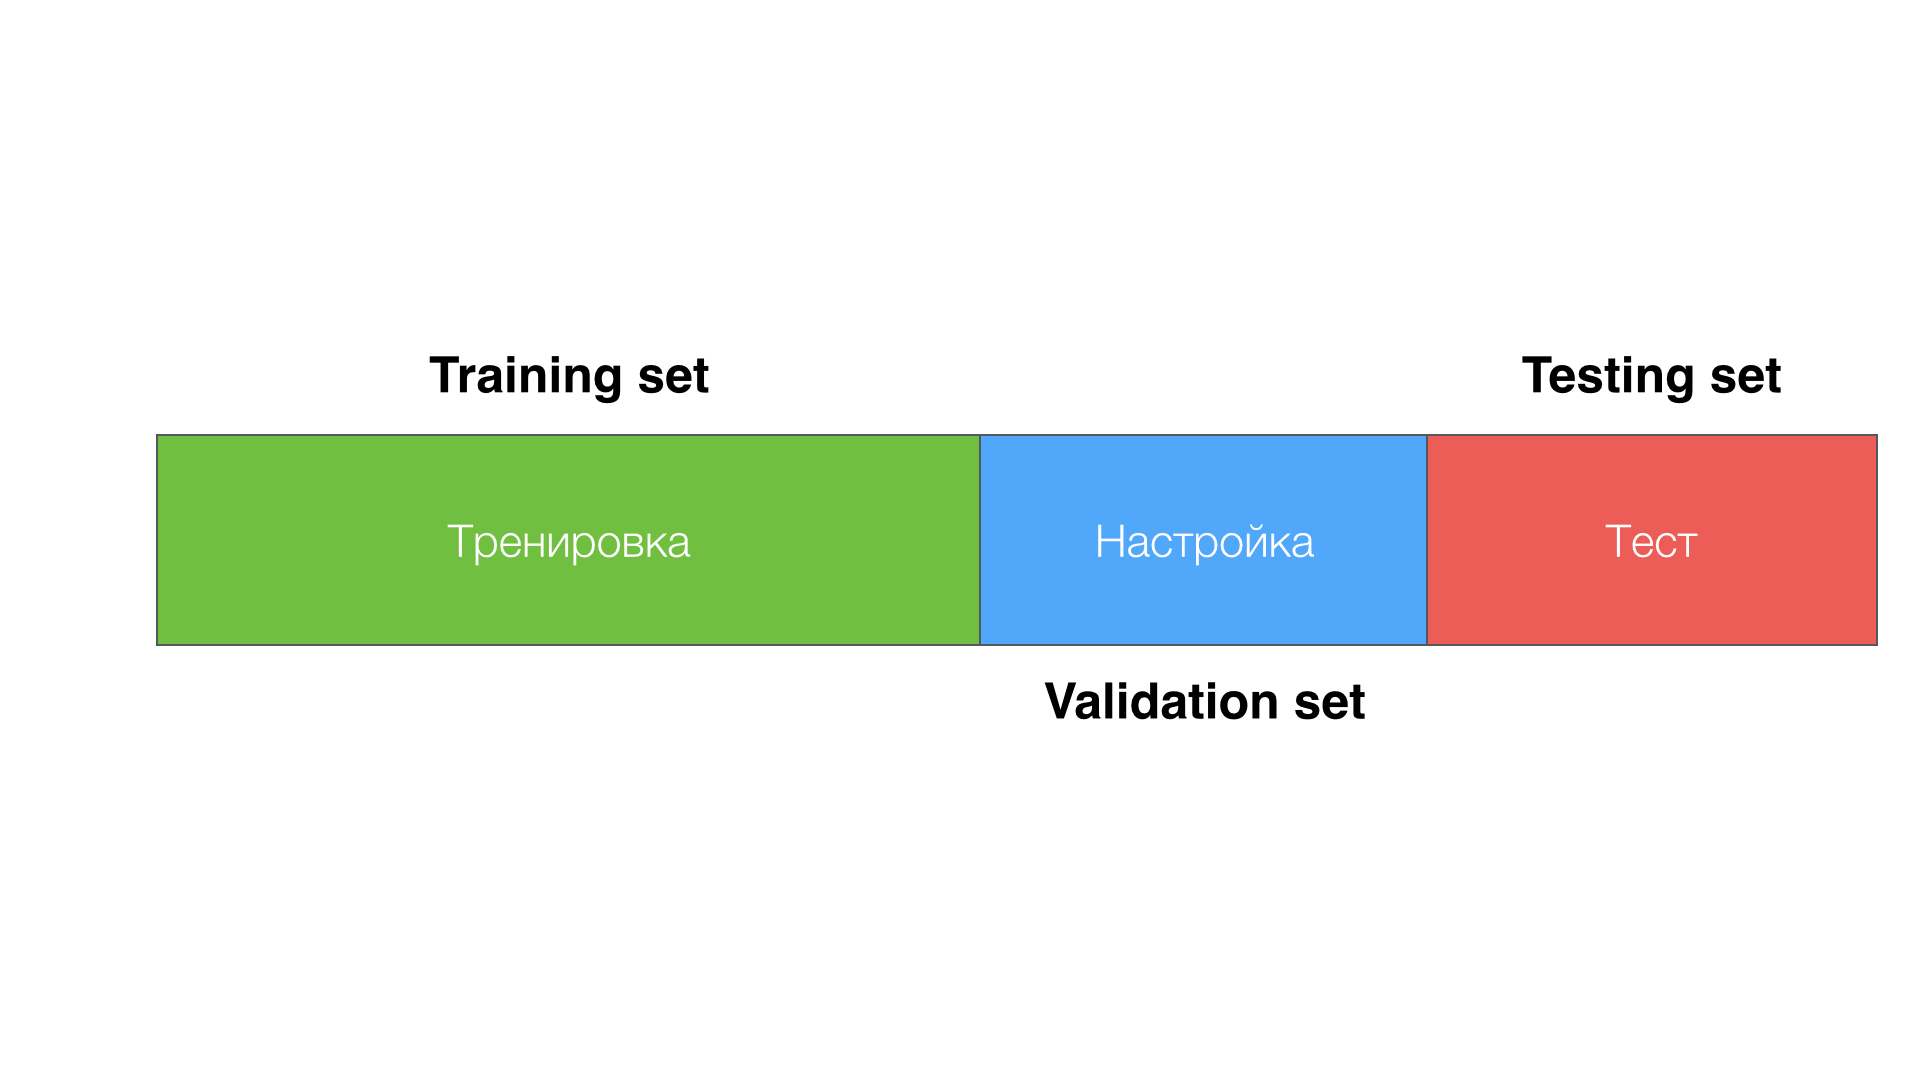
\includegraphics[scale=0.15]{images/vtt.png}
\end{center}
  
 \end{frame}
 
% ============================================== %

\begin{frame}{Решение 2: скользящий контроль}

(n-times) (stratified) cross-validation

\begin{center}
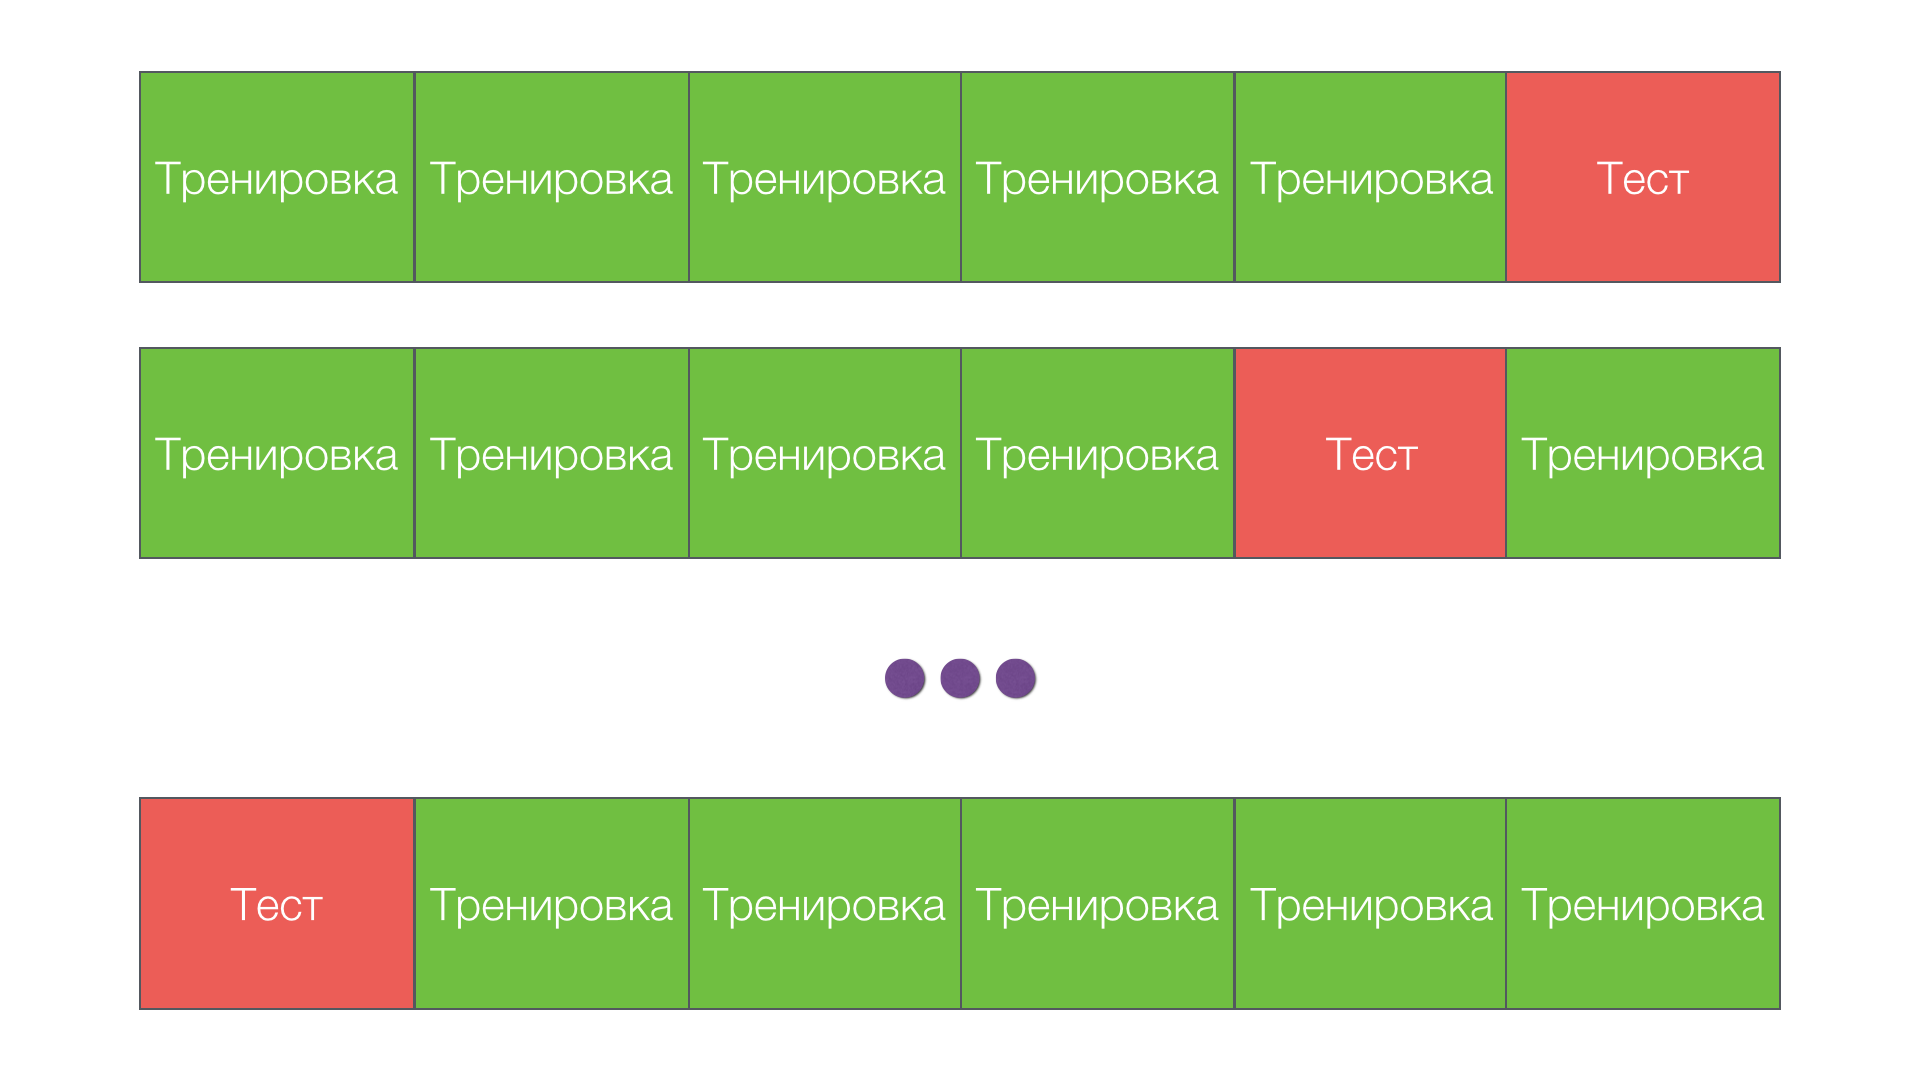
\includegraphics[scale=0.15]{images/cv.png}
\end{center}

частный случай: leave-one-out
  
 \end{frame}
 
 % ============================================== %

\begin{frame}{Решение 3: bootstrap}

выбираем в тренировочную выбоку $n$ объектов с возвращением

\begin{center}
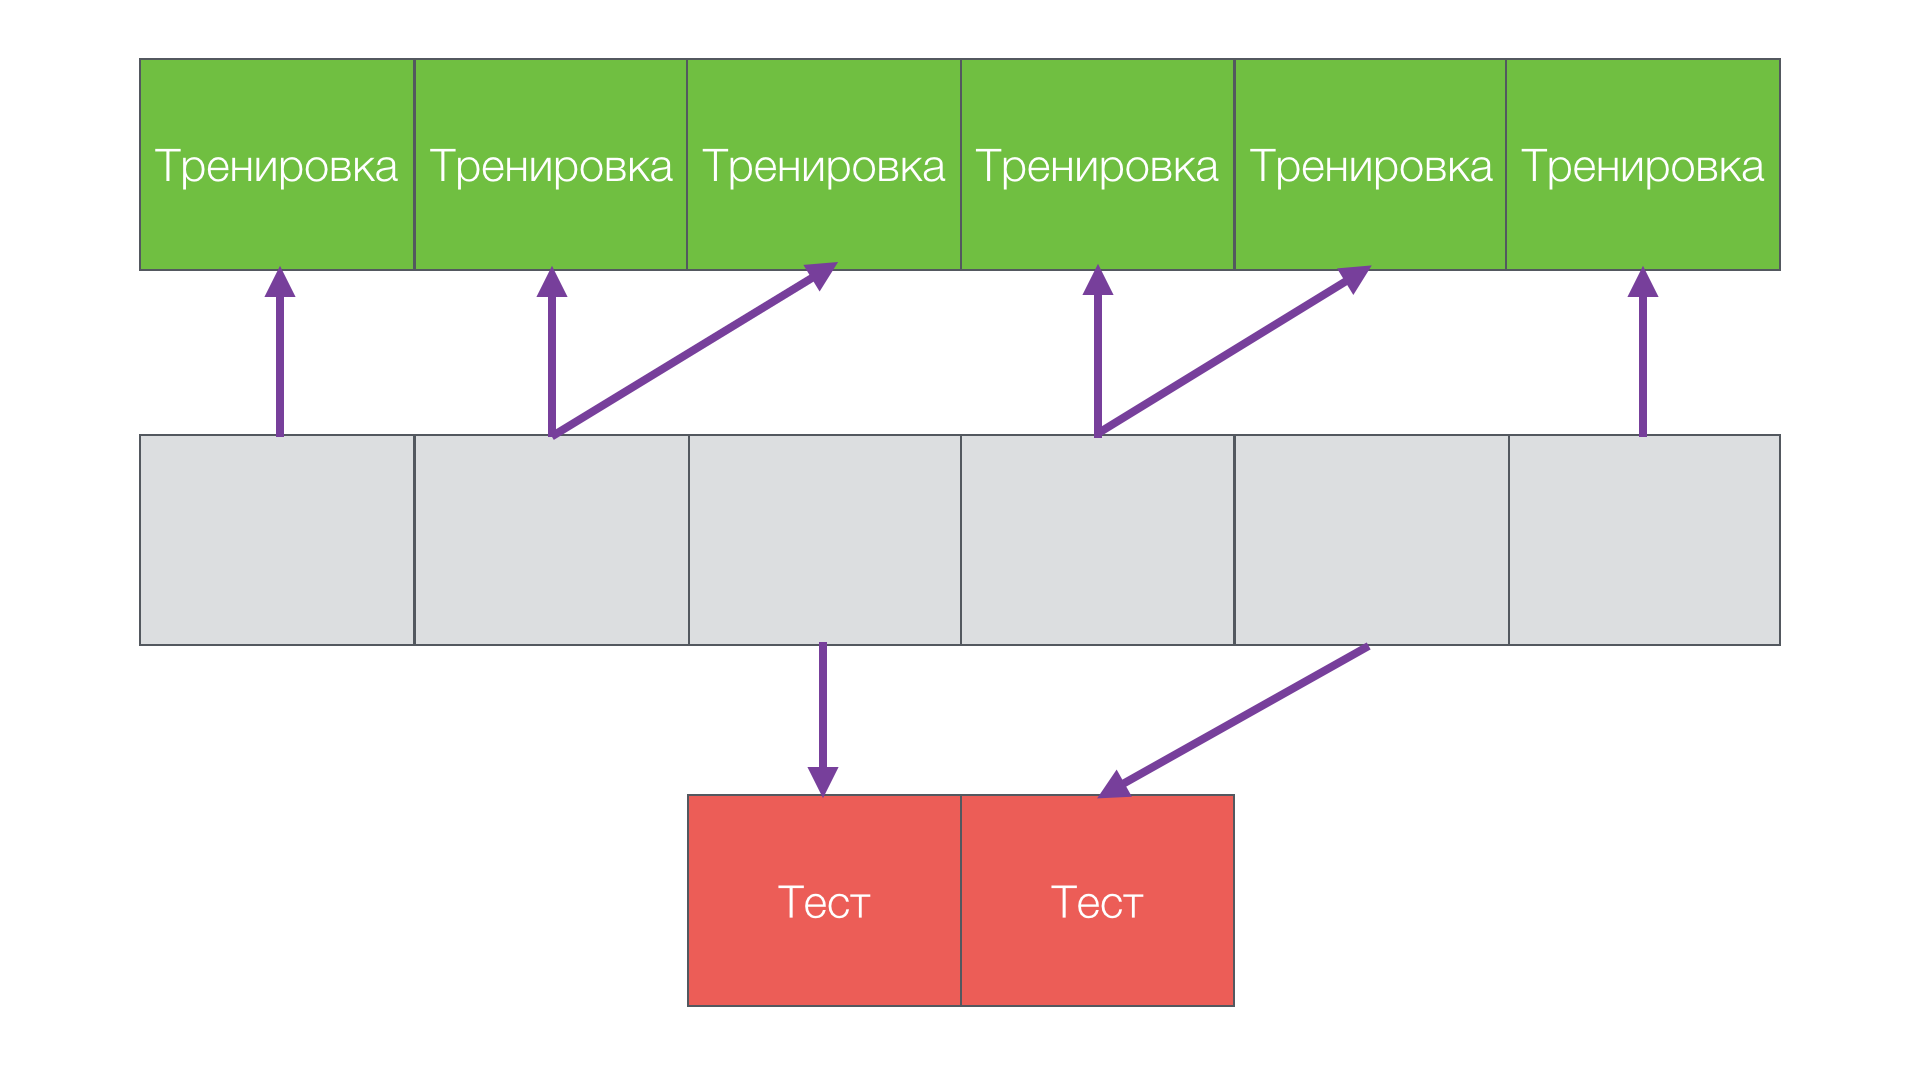
\includegraphics[scale=0.15]{images/boot.png}
\end{center}

упражнение: найти математическое ожидание размера тестовой выборки.
  
\end{frame}

% ============================================== %

\begin{frame}{Доверительный интервал для success rate}

При тестировании на $N=100$ объектах было получено $25$ ошибок. Таким образом измеренная вероятность успеха (success rate) составила $f=0.75$. Найти доверительный интервал для действительной вероятности успеха c уровнем доверия $\alpha=0.8$. 

\begin{exampleblock}{Решение}
Пусть $p$ -- действительная вероятность успеха в испытаниях бернулли, тогда
\[
f \sim \mathcal{N}\left( p, p(1-p)/N \right).
\]
Воспользовавшись табличным значением $P(-z \leq \mathcal{N}(0,1) \leq z) = \alpha$, имеем
\[
P\left(-z \leq \frac{f-p}{\sqrt{p(1-p)/N}} \leq z \right) = \alpha,
\]
откуда
\[
p \in \left(f + \frac{z^2}{2N} \pm z \sqrt{\frac f N - \frac{f^2}{N}+\frac{z^2}{4N^2}} \right)/\left(1 + \frac {z^2}{N} \right) = [0.69, 0.80]
\]
\end{exampleblock}
  
 \end{frame}
 
% ============================================== %

\begin{frame}{Метрики качества. Вероятностные модели.}

Пусть $t_i$ - действительный класс для объекта $x_i$
\begin{itemize}
\item  Information loss 
\[
- \frac 1 N \sum_i \log_2 p(t_i | x_i)
\]
\item Quadratic loss 
\[
\frac 1 N \sum_j (p(t_j | x_i) - a_j(x_i))^2,
\] 
где
\[
a_j(x_i) = \begin{cases}
1, \;\text{если}\;C_j = t_i\\
0, \;\text{иначе}
\end{cases} 
\]
\end{itemize}

\end{frame}

% ============================================== %

\begin{frame}{Метрики качества. Функции решения.}

\begin{center}
\begin{tabular}{|c r | c c|}
\cline{3-4}
 \multicolumn{2}{c|}{} & \multicolumn{2}{c|}{Предсказанный} \\
 \cline{3-4}
 \multicolumn{2}{c|}{} & {\bf true} & {\bf false} \\
 \hline
 \multirow{2}{*}{Действительный} & \multicolumn{1}{|c|}{\bf true} & TP & FN \\
 & \multicolumn{1}{|c|}{\bf false}  & FP & TN \\
 \hline
\end{tabular}
\end{center}

\[
success\;rate = accuracy = \frac{TP + TN}{TP + FP + FN + TN}
\]
\[
recall = TPR = \frac{TP}{TP + FN};\;\;precision = \frac{TP}{TP + FP}
\]
\[
FPR = \frac{FP}{FP + TN}
\]
\[
affinity = lift = \frac{accuracy}{p}
\]

\end{frame}

% ============================================== %

\begin{frame}{Receiver Operating Characteristic}

\[
TPR = \frac{TP}{TP + FN};\;\;FPR = \frac{FP}{FP + TN}
\]

\begin{center}
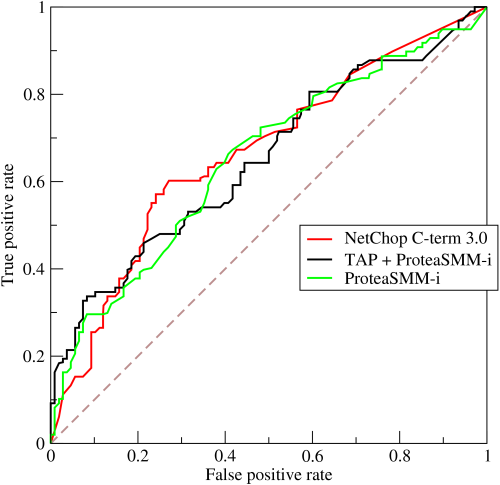
\includegraphics[scale=2.0]{images/roc.png}
\end{center}

\end{frame}

% ============================================== %

\begin{frame}{Упражнение}

\begin{exampleblock}{Простые классификаторы}
В генеральной совокупности существуют объекты 3 классов, вероятность появления которых $p_1 < p_2 < p_3$. Первый классификатор относит все объекты к классу с большей вероятностью (то есть к третьему). Второй классификатор случайно относит объект к одному из классов в соответствии с базовым распределением. Рассчитать precision и recall, которые эти классификаторы дают для каждого из 3 классов.
\end{exampleblock}

\end{frame}

% ============================================== %

\begin{frame}{Метрики качества. Регрессия}

\[
MSE = \frac 1 N \sum (y(x_i) - t_i)^2, \;\; RMSE = \sqrt{MSE}
\]
\[
MAE =  \frac 1 N \sum |y(x_i) - t_i|, \;\; RMAE = \sqrt{MAE}
\]
\[
RSE =  \frac{\sum (y(x_i) - t_i)^2}{\sum (t_i - \bar{t})^2}
\]
\[
correlation = \frac{S_{ty}}{S_t S_y};\;\; S_{ty} = \frac{\sum(y(i)-\overline{y(i)})(t_i - \bar t)}{N-1}
\]
\[
S_{y} = \frac{\sum(y(i)-\overline{y(i)})^2}{N-1};\;\;S_{t} = \frac{\sum(t_i - \bar t)^2}{N-1}
\]

\end{frame}

% ============================================== %

\begin{frame}{MDL принцип: интуиция}

\begin{center}
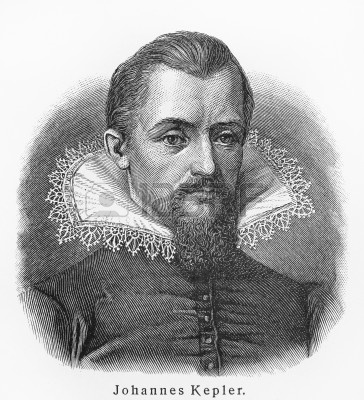
\includegraphics[scale=0.35]{images/kepler.jpg}
\vspace{0.1em}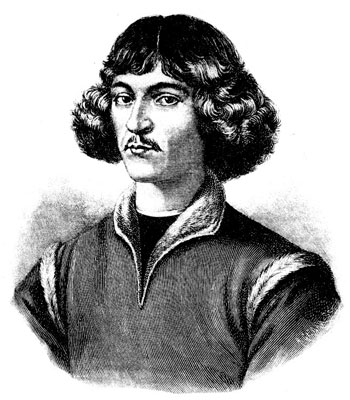
\includegraphics[scale=0.37]{images/copernicus.jpg}
\end{center}

\end{frame}

% ============================================== %

\begin{frame}{Спасибо!}

\begin{center}
{\Large Обратная связь}
\end{center}

\end{frame}

\end{document}